\documentclass[a4paper,12pt]{article}
\usepackage[russian]{babel}

% Самые необходимые пакеты
\usepackage[T2A]{fontenc}
\usepackage[utf8]{inputenc}
\usepackage[russian]{babel}
\usepackage{geometry}
\usepackage{amsmath}
\usepackage{graphicx}
\usepackage{float} 
\usepackage{xcolor}
\usepackage{listings}
\usepackage{hyperref}
\usepackage{array}
\usepackage{caption}
\usepackage{booktabs}
\usepackage{amssymb}
\usepackage{subcaption}
\usepackage{caption}
\captionsetup[figure]{name=Рисунок}
\captionsetup[table]{name=Таблица}
\usepackage{pgfplots}
\pgfplotsset{compat=1.18}
\usetikzlibrary{arrows.meta}
\usepackage{capt-of}
\usepackage{multirow}


\lstset{
	language=Matlab,
	basicstyle=\ttfamily\small,
	keywordstyle=\color{blue}\bfseries,
	commentstyle=\color{gray}\itshape,
	stringstyle=\color{red},
	numberstyle=\tiny\color{gray},
	numbers=left,
	stepnumber=1,
	numbersep=8pt,
	backgroundcolor=\color{white},
	frame=single,
	breaklines=true,
	breakatwhitespace=true,
	tabsize=4,
	showspaces=false,
	showstringspaces=false,
	captionpos=b,
	escapeinside={\%*}{*)}, % для вставки LaTeX кода внутри листинга
}
% Настройка геометрии
\geometry{left=1.5cm, right=2cm, bottom=2cm, top=2cm}

\begin{document}
	
	% Титульный лист
	\begin{titlepage}
		\centering
		\vspace*{1cm}
		
		% Министерство
		{\small
			Министерство науки и высшего образования Российской Федерации\\
			Федеральное государственное автономное образовательное учреждение\\
			высшего образования\\
			«Национальный исследовательский университет ИТМО»\\
		}
		
		\vspace{2cm}
		
		% Факультет
		{\large
			Факультет систем управления и робототехники\\
		}
		
		\vspace{3cm}
		
		% Основной заголовок
		{\Huge\bfseries
			ОТЧЕТ\\
		}
		\vspace{0.5cm}
		{\LARGE\bfseries
			о лабораторной работе №4\\
		}
		
		\vspace{1cm}
		
		% Дисциплина и тема
		{\Large
			По дисциплине: «Линейные системы автоматического управления»\\
			\vspace{0.5cm}
			Тема: «Точностные свойства системы, астатизмы и регуляторы»\\
		}
		
		\vspace{3cm}
		
		% Информация о студенте и преподавателях
		\begin{minipage}{0.4\textwidth}
			\raggedright
			{\large
				Студент:\\
			}
			Охрименко Е. Д.\\
			Поток: 1.1.3\\
			Вариант: 17\\
		\end{minipage}
		\hfill
		\begin{minipage}{0.4\textwidth}
			\raggedleft
			{\large
				Преподаватель:\\
			}
			Пашенко А. В.\\
		\end{minipage}
		
		\vfill
		
		% Город и год
		{\large
			Санкт-Петербург\\
			2025\\
		}
		
	\end{titlepage}
	
	\newpage
	\tableofcontents
	
	\newpage
	\section{Задание. Задача стабилизации с идеальным дифференцирующим звеном}

	
	Рассмотрю линейную систему второго порядка, заданную уравнением:
	
	\[
	a_2 \ddot{y} + a_1 \dot{y} + a_0 y = u(t)
	\]
	
	Требуется:
	
	\begin{itemize}
		\item Задать коэффициенты \( a_2, a_1, a_0 \), обеспечивающие наличие хотя бы одного неустойчивого полюса.
		\item Смоделировать свободное движение разомкнутой системы при начальных условиях \( y(0) = 0 \), \( \dot{y}(0) \ne 0 \).
		\item Ввести регулятор \( u = k_0 y + k_1 \dot{y} \), построить структурную схему замкнутой системы.
		\item Определить условия устойчивости замкнутой системы и подобрать параметры \( k_0 \), \( k_1 \), обеспечивающие асимптотическую устойчивость.
		\item Выполнить моделирование замкнутой системы и сравнить её поведение с разомкнутой.
	\end{itemize}
	
	
	\subsection{Характеристическое уравнение и график свободного движения}
	
	Запишу характеристическое уравнение системы (при \( u(t) = 0 \)):
	
	\[
	a_2 \lambda^2 + a_1 \lambda + a_0 = 0
	\]
	
	Для обеспечения неустойчивости системы выберу следующие корни характеристического уравнения системы: 
	\[
	\begin{cases}
		\lambda_1 = 1 \\
		\lambda_2 = -2
	\end{cases}
	\]
	
	
	Подставлю корни в уравнение, чтобы получить характеристический многочлен:
	
	\[
	(\lambda - 1)(\lambda + 2) = \lambda^2 + 1\lambda - 2
	\]
	
	Найду коэффициенты:
	\[
	\begin{cases}
		a_2 = 1 \\
		a_1 = 1 \\
		a_0 = -2
	\end{cases}
	\]
	
	Таким образом, исходное уравнение примет вид:
	
	\[
	\ddot{y} + 1 \dot{y} - 2 y = u(t)
	\]
	
	Также выберу начальные значения для моделирования свободного движения системы:
	
	\[
	\begin{cases}
		y(0) = 0 \\
		\dot{y}(0) = -1
	\end{cases}
	\]
	
	Выполню моделирование свободного движения разомкнутой системы \(y_\text{раз}(t)\).
	
	\begin{figure}[H]
		\centering
		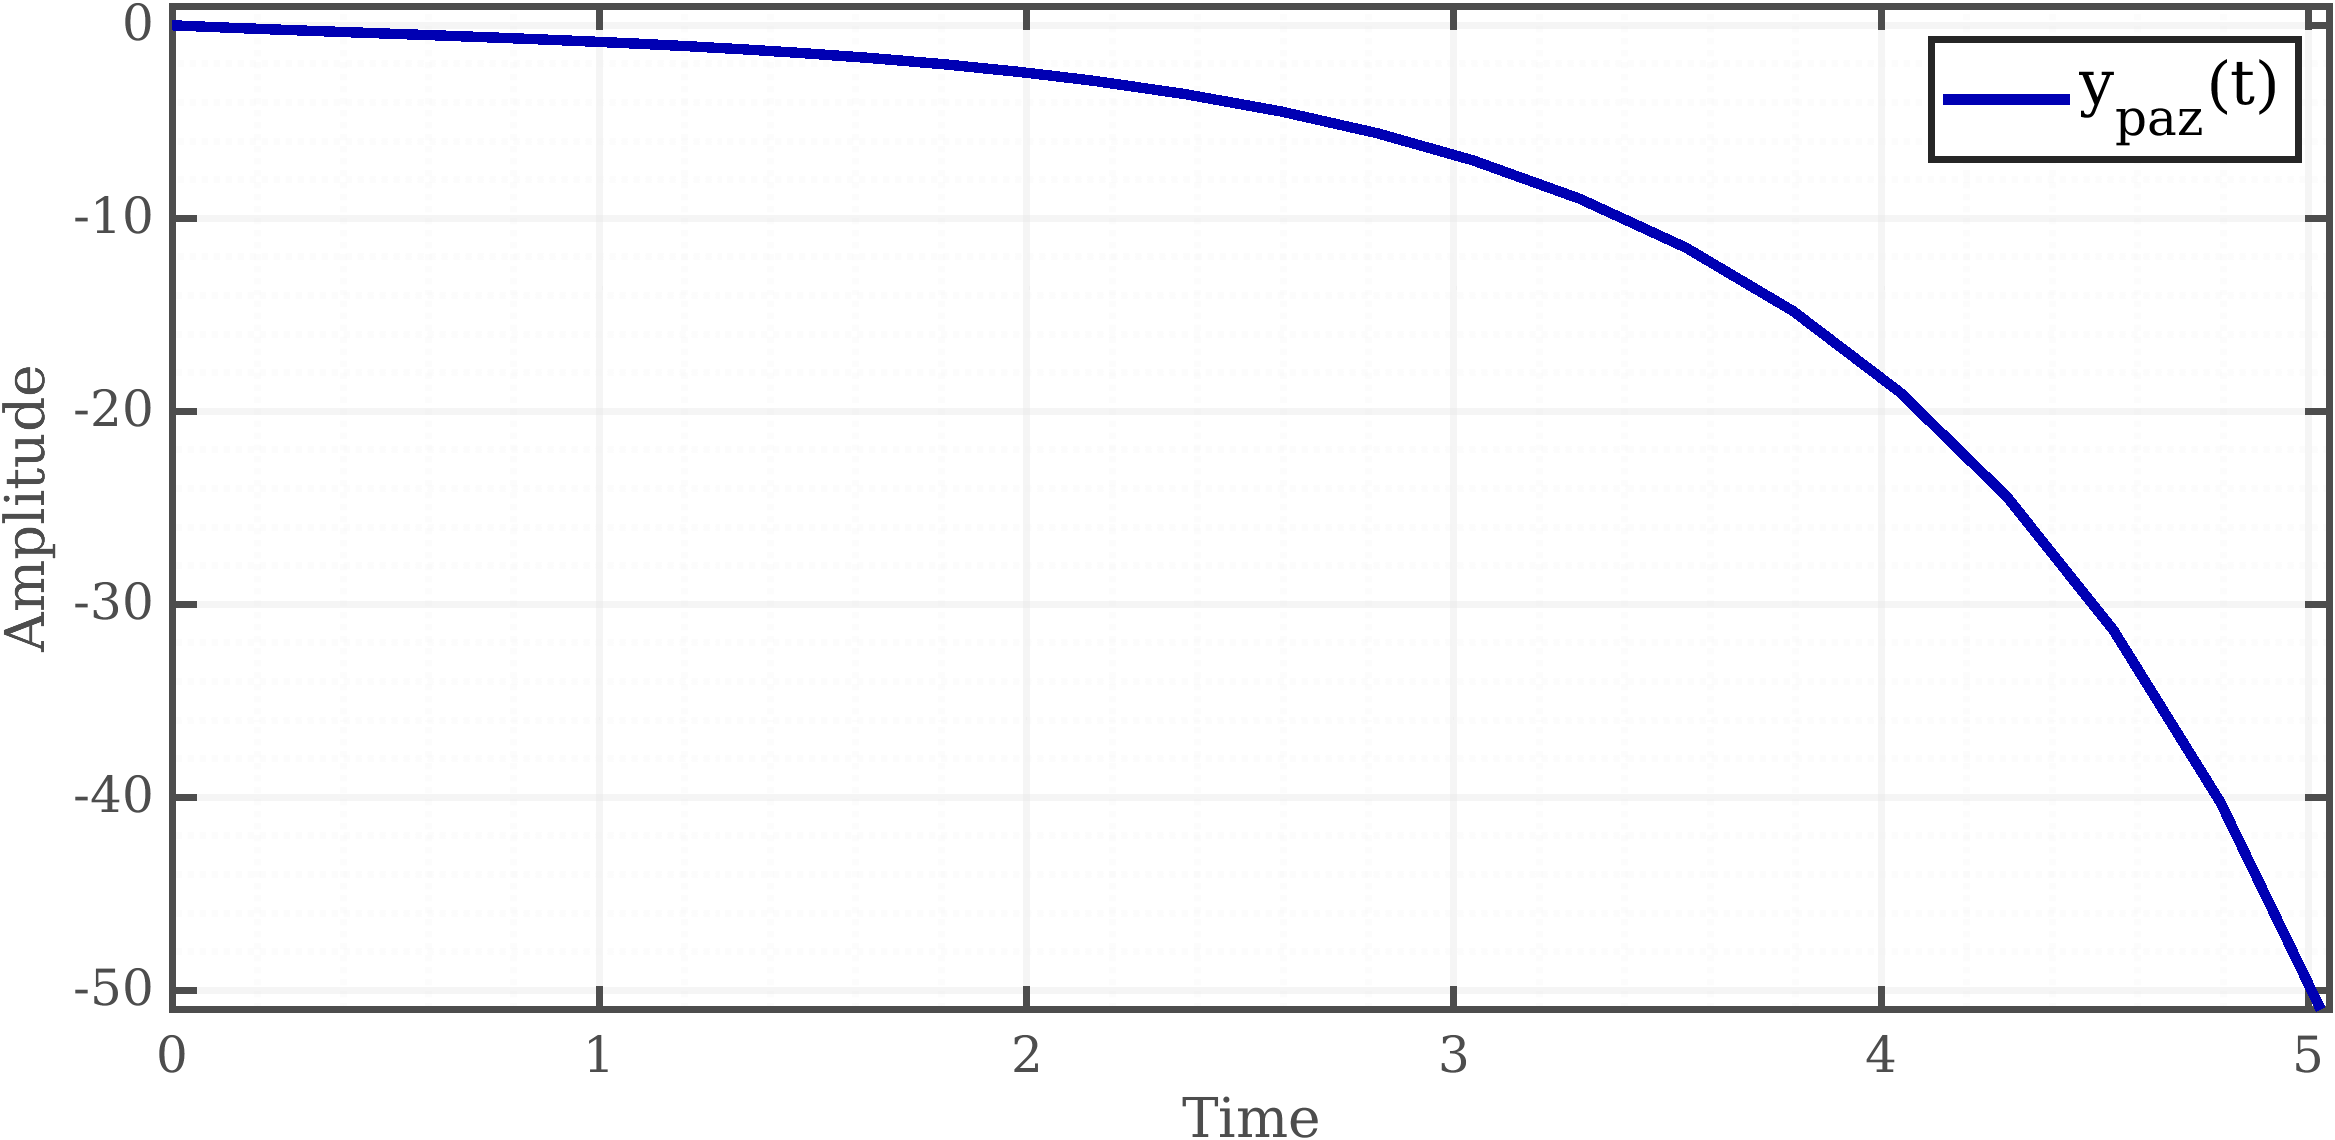
\includegraphics[width=1\textwidth]{../images/task1/y_raz.png}
		\caption{График выхода \( y_{\text{раз}}(t) \)}
	\end{figure}
	
	Система неустойчива.
	
	\subsection{Регулирование и стабилизация системы}
	
	Далее рассмотрю регулятор: \[u = k_0 y + k_1 \dot{y}\]
	
	И определю при каких значениях параметров \(k_0\) и \(k_1\) система будет устойчивой. Подставлю регулятор в уравнение объекта управления:
	
	\[
	\ddot{y} + 1 \dot{y} - 2 y = k_0 y + k_1 \dot{y} = u
	\]
	
	\[
	\ddot{y} + 1 \dot{y} - k_1 \dot{y} - 2 y - k_0 y  = 0
	\]

	\[
	\ddot{y} + (1 - k_1) \dot{y} - (2 - k_0) y = 0
	\]
	
	Запишу характеристическое уравнение для замкнутой системы:
	\[
	\lambda^2 + (1 - k_1) \lambda - (2 - k_0) = 0
	\]
	
	Для устойчивости системы необходимо, чтобы все корни уравнения имели отрицательную действительную часть. Воспользуюсь критерием Гурвица:
	
	\[
	\begin{cases}
		1 - k_1 > 0 \\
		-2 - k_0 > 0 \\
	\end{cases}
		\quad \Longrightarrow \quad
	\begin{cases}
		k_1 < 1 \\
		k_0 < -2 \\
	\end{cases}
	\]

	
	Для обеспечения устойчивости замкнутой системы выберу параметры регулятора \(k_0\) и \(k_1\) из получившихся диапазонов: 
	
	\[
	\begin{cases}
		k_1 = -3 \\
		k_0 > -5 \\
	\end{cases}
	\]
	
	
	
	
	
	
	
	
	
	
	
	
	
	
	
	
	\newpage
	\section{Вывод}
	
	
	Материалы работы: \href{https://github.com/decadeos/ITMO/tree/master/3_course/lsau/lab3}{\texttt{github.com}}
	
\end{document}